% !TeX root = RJwrapper.tex
\title{Visual diagnostics for constrained optimisation with application to
guided tours}
\author{by H.Sherry Zhang}

\maketitle

\abstract{%
Projection pursuit searches for interesting low-dimensional views of
high-dimensional data via the optimisation of an index function. The
initial paper by Friedman \& Tukey in 1974 stated that ``the technique
used for maximising the projection index strongly influences both the
statistical and the computational aspects of the procedure.'' However,
while many projection pursuit indices have been proposed in the
literature, less work has been done on the optimisation procedures. In
this paper we introduce visual diagnostics for optimisation algorithms,
in particular those available in the projection pursuit guided tour.
These diagnostics and workflows can be applied to a broad class of
optimisers, to assess their performance. An R package, ferrn, has been
created to implement the diagnostics.
}

\hypertarget{introduction}{%
\section{Introduction}\label{introduction}}

Visualisation is widely used in exploratory data analysis
\citep{tukey1977exploratory}. Presenting information in a graphical
format often allows people to uncover information they would otherwise
not be aware of and provides a more comprehensive understanding of the
problem at hand. The work presented in this paper combines data
visualization with optimization methods. It aims at bring visualization
tools into optimization problems to assist users to better understand
the performance of their optimization methods in practice. This
motivates our work of creating plots to diagnose optimisation algorithms
which in turn can be also used not only to understand optimization
performance but also to understand and compare the behaviour of
different algorithms.

The goal of continuous optimisation is to find the best solution within
the space of all feasible solutions where typically the best solution is
decided by an objective function. Broadly speaking optimization can be
unconstrained or constrained \citep{kelley1999iterative}. The
unconstrained problem can be formulated as a minimization (or
maximization) problem such as \(\min_{x} f(x)\) where
\(f:\mathbb{R}^n \rightarrow \mathbb{R}\) is an objective function with
certain properties defined in an \(L^p\) space. In this case, solutions
rely on gradient descent or ascent methods. In the constrained
optimization problem additional restrictions are introduced via a set of
functions that can be convex or non-convex:
\(g_i:\mathbb{R}^n \rightarrow \mathbb{R}\) for \(i = 1, \ldots k\) and
hence the problem can be written as \(\min_{x} f(x)\) \emph{subject to}
\(g_i(x) \leq 0\). Here methods such as Langrange multipliers and convex
optimization methods including linear and quadratic programming can be
used.

The motivation of this paper is the optimisation problem arising in the
projection pursuit guided tour \citep{buja2005computational} which is an
exploratory data analysis tool that is defined to detect
\emph{interesting structures} or features in high-dimensional data
through a set of lower-dimensional projections that cover the entire
high dimensional space using interpolation methods called tours
\citep{cook2008grand}. The target of the optimisation is to identify the
most \emph{interesting} low-dimensional views of the data given by a
corresponding projection matrix. The most \emph{interesting} structures
are formally defined by a function of projections, called index function
which is optimized to uncover the most reveling structures in a high
dimensional space \citep{cook1993projection}.

The optimization challenges encountered in the projection pursuit guided
tour problem are common to those of optimization in general. Examples of
those include the existence of multiple maxima (local and global), the
trade off between computational burden and proximity to the maxima,
dealing with noisy objective functions that might be non smooth and non
diferentiable \citep{jones1998efficient}. Those are not unique to this
context and therefore the visualization tools and optimization methods
presented in this paper can be easily apply to any other optimization
problems.

The remainder of the paper is organised as follows. Section \ref{optim}
provides an overview of optimisation methods, specifically line search
methods. Section \ref{tour} reviews projection pursuit guided tour,
defines the optimisation problem and introduces three existing
algorithms. Section \ref{vis-diag} presents the new visual diagnostics.
A data structure is defined to capture information during the
optimisation, and used in different types of diagnostic plots. Section
\ref{application} shows applications of how these plots can be used to
understand and compare different algorithms. We also discuss how these
insights contribute to modifications that improve the algorithms.
Finally, Section \ref{implementation} describes the R package: ferrn,
that implements the visual diagnostics.

\hypertarget{optim}{%
\section{Optimisation Methods}\label{optim}}

Optimization problems are ubiquitous in many areas of study. While in
some cases, analytical solutions can be found, the majority of problems
rely on numerical methods to find the optimal solution. These numerical
methods follow interactive approaches that aim at finding the optimum by
progressively improving the current solution until a desirable accuracy
is achieved. Although that principle seems uncomplicated, optimization
methods need to deal with many challenges such as the existence of
multiple maxima (local and global), the trade off between desirable
accuracy and computational burden, as well as dealing with noisy
objective functions and possible constraints. In addition, optimization
results might depend on the algorithm starting values affecting the
consistency of results.

Our interest is on constrained optimization (REF) as defined in the
introduction section and assume that it is not possible to find a
solution to the problem in the way of a closed form. That is, the
problem consists of finding the minimum or maximum of a function
\(f \in L^p\) in the constrained \(\mathbb{A}\) space.

Optimization methods can be divided in various classes (REF). In this
paper, we focused on methods that rely on the objective function
derivatives known as gradient methods, and those which are known as
derivative free methods where optimization does not rely on the gradient
or derivatives information.

In gradient descent methods the goal is to find the minimum of an
objective function while in gradient ascent methods the interest is in
the maximum. The minimum is searched for by taken steps proportional to
the negative gradient or of the function at the evaluation point
(analogously positive gradient for gradient ascent methods), that is
\(x_{k+1} = x_k -\alpha_kS_k\) where \(\alpha_k\) is the step size or
the learning rate \citep{fletcher2013practical}. The step size is the
key in the success of the optimization problem as inadequate step sizes
might lead to a failure in convergence. These methods are known to be
relative slow and can have convergence issues when problems are poorly
conditioned \citep{trefethen1997numerical}. In order to solve some of
those problems, line minimization or line search methods were proposed
\citep{shi2004convergence} where the step size is chosen in such a way
that convergence is ensured. In line search methods users are required
to provide an initial estimate \(x_{1}\), a search direction \(S_k\) for
each iteration where the objective is to find the value of
\(\alpha_k \in \mathbb{R}\) that minimizes \(f(x_k + \alpha_kS_k)\) with
respect to \(\alpha_k\) (this step is called the line search). Then move
on to the next point following \(x_{k+1} = x_k + \alpha_kS_k\) and
repeat the process until the desire convergence is reached. Modern
development of line search methods focuses on improving the computation
of the searching direction \(S_{k}\), and on approximations of the step
size \(\alpha_k\) together with reducing the computational storing
burden of the intermediate computations while catering for practical
optimisation problems. In the next section two line search methods for
the optimisation used in the projection pursuit guided tour will be
presented.

Although gradient optimization methods are very popular, they rely on
the existence of the objective function derivatives and on the
complexity of the constraints. Because of that, the second big class of
optimization problems look at derivative free methods where the emphasis
is on finding, in most cases, a near optimal solution. Examples of those
include response surface methodology \citep{box1951experimental},
stochastic approximation \citep{robbins1951stochastic}, random search
\citep{fu2015handbook} and heuristic methods
\citep{sorensen2013metaheuristics}. Later, we will present an
optimization algorithm within the random search class, namely simulated
annealing for optimization with the guided tour. Moreover, we will
introduce an algorithm to further improve optimization solutions both in
gradient descent methods and in derive free optimization.

Several R implementations address optimization problems with both
general purpose as well as tasks specifics solvers. The most prominent
one within the general solvers is \texttt{optim()} in the package
\CRANpkg{stats}\citep{stats} which have functions for gradient based and
derivative free methods. Other packages having similar functionalities
include \CRANpkg{nloptr}.

\hypertarget{tour}{%
\section{Projection pursuit guided tour}\label{tour}}

The projection pursuit guided tour combines two different methods in
exploratory data analysis, focusing on different aspects. Projection
pursuit, coined by \citet{friedman1974projection}, detects interesting
structures (e.g.~clustering, outliers and skewness) in multivariate data
via low dimensions projection. The guided tour is using ideas from
projection pursuit to define a particular variation in a broader class
of data visualisation methods, building on the grand tour approach
\citep{As85}.

To define projection pursuit, we first need to establish the notation
used. Let \(\mathbf{X}_{n \times p}\) be the data matrix, with \(n\)
observations in \(p\) dimensions. A d-dimensional projection can be seen
as a linear transformation from \(\mathbb{R}^p\) into \(\mathbb{R}^d\),
and defined as \(\mathbf{Y} = \mathbf{X} \cdot \mathbf{A}\), where
\(\mathbf{Y}_{n \times d}\) is the projected data and
\(\mathbf{A}_{p\times d}\) is the projection matrix. Define
\(f: \mathbb{R}^{n \times d} \mapsto \mathbb{R}\) to be an index
function that maps the projected data \(\mathbf{Y}\) (corresponding to
an associated projection matrix \(\mathbf{A}\)) onto an index value
\(I\) (QUESTION: Isn't f the index function?). This is commonly known as
the projection pursuit index function, or just index function, and is
used to measure the ``interestingness'' of a given projection.

A number of index functions have been proposed in the literature to
detect different data structures, including Legendre index
\citep{friedman1974projection}, Hermite index
\citep{hall1989polynomial}, natural Hermite index
\citep{cook1993projection}, chi-square index
\citep{posse1995projection}, LDA index \citep{lee2005projection} and PDA
index \citep{lee2010projection}.

As a general visualisation method, a tour produces animations of high
dimensional data via rotations between low dimension planes. Different
tour types choose these planes differently, for example, a grand tour
\citep{cook2008grand} selects the planes randomly and a manual tour
\citep{cook1997manual} gradually phases in and out one variable, to
understand the contribution of that variable in the projection. Guided
tour, the main interest of this paper, chooses planes with the aid of
projection pursuit. Given a random start, projection pursuit iteratively
finds bases with higher index values and the guided tour constructs the
geodesic interpolation between these planes to form a tour path.

Mathematical details of the geodesic interpolation can be found in
\citet{buja2005computational}. Figure \ref{fig:tour-path} shows a sketch
of the tour path. The blue frames are produced by the projection pursuit
optimisation algorithm, and the white frames interpolate between them.
The tour method has been implemented in the R package \CRANpkg{tourr}
\citep{tourr}, available on the Comprehensive R Archive Network at
\url{https://cran.r-project.org/web/packages/tourr/}

\begin{Schunk}
\begin{figure}

{\centering 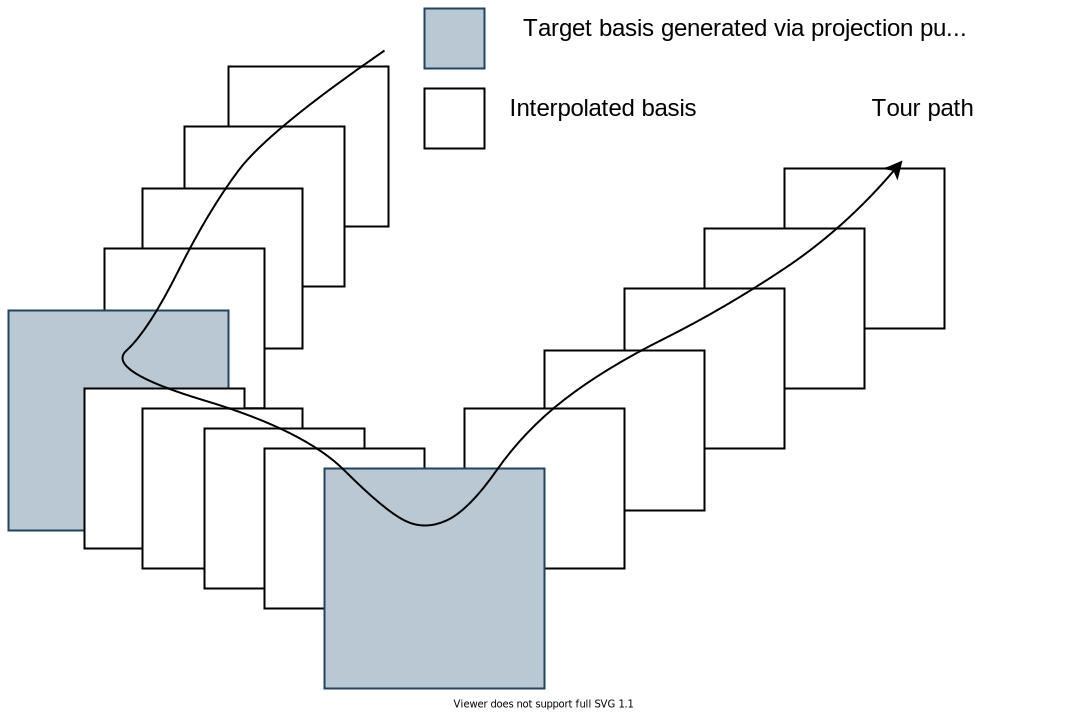
\includegraphics[width=0.5\linewidth,height=0.25\textheight]{/Users/hzha400/Documents/PhD/research/paper-tour-vis/img/tour_path} 

}

\caption[Each square (frame) represents the projected data with a corresponding basis]{Each square (frame) represents the projected data with a corresponding basis. Blue frames are found by an optimisation algorithm iteratively whilst the white frames are constructed between two blue frames by geodesic interpolation.}\label{fig:tour-path}
\end{figure}
\end{Schunk}

\hypertarget{tour-optim}{%
\subsection{Optimisation in the tour}\label{tour-optim}}

pa The optimisation problem in the tour context is stated as follows:
\ldots. .Given a randomly generated starting basis \(\mathbf{A}_1\),
projection pursuit finds the final projection basis \(\mathbf{A}_T\)
that satisfies the following optimisation problem:

\begin{align}
&\arg \max_{\mathbf{A} \in \mathcal{A}} f(\mathbf{X} \cdot \mathbf{A}) \\
&s.t.  \mathbf{A}^{\prime} \mathbf{A} = I_d
\end{align}

\noindent where \(I_d\) is the \(d\)-dimensional identity matrix and the
constraint requires the projection bases \(\mathbf{A}\) to be orthogonal
matrices.

Several features of this optimisation are worth noticing. First of all,
this is a constrained optimisation problem as the decision variables
form the entries of a projection basis, which is required to be
orthonormal. It is also likely that the objective function may not be
differentiable for a constructed index function and in these cases,
gradient-based methods may not work well. Although finding the global
maximum is the goal of an optimisation problem, it is also interesting
to inspect local maximum in projection pursuit since it could present
unexpected interesting projections. Lastly, there is also one
computational consideration: the optimisation procedure needs to be fast
to compute since the tour animation is played in real-time.

\hypertarget{existing-algorithms}{%
\subsection{Existing algorithms}\label{existing-algorithms}}

Below we introduce three possible algorithms: \texttt{search\_better},
\texttt{search\_better\_random}, and \texttt{search\_geodesic}. The
first two are derivative free methods that sample candidate bases in the
neighbourhood whilst \texttt{search\_geodesic} is an analogue of
gradient ascent on the projection basis space.

\begin{algorithm}
\SetAlgoLined
  \SetKwInOut{Input}{input}
  \SetKwInOut{Output}{output}
    \Input{$\mathbf{A}_{\text{cur}}$, $f$, $\alpha$, $l_{\max}$} 
    \Output{$\mathbf{A}_{l}$}
  initialisation\;
  Set $l = 1$\;
  \While{$l < l_{\max}$}{
    Generate $\mathbf{A}_{l} = (1- \alpha)\mathbf{A}_{\text{cur}} + \alpha \mathbf{A}_{\text{rand}}$ and orthogonalise $\mathbf{A}_{l}$\;
    Compute $I_{l}  = f(\mathbf{A}_{l})$\;
    \If{$I_{l} > I_{\text{cur}}$}{
      \KwRet{$\mathbf{A}_{l}$} \;
      }
    $l = l + 1$\;
  }
  \caption{random search}
  \label{random-search}
\end{algorithm}

\texttt{search\_better} is a random search device that samples a
candidate basis \(\mathbf{A}_{l}\) in the neighbourhood of the current
basis \(\mathbf{A}_{\text{cur}}\) by
\(\mathbf{A}_{l} = (1- \alpha)\mathbf{A}_{\text{cur}} + \alpha \mathbf{A}_{\text{rand}}\)
where \(\alpha\) controls the radius of the sampling neighbourhood and
\(\mathbf{A}_{\text{rand}}\) is a randomly generated matrix with the
same dimension as \(\mathbf{A}_{\text{cur}}\). \(\mathbf{A}_{l}\) is
then orthogonalised to ensure the orthonormal constraint is fulfilled.
When a basis is found with index value higher than the current basis
\(\mathbf{A}_{\text{cur}}\), the search terminates and outputs the basis
for guided tour to construct an interpolation path. The next iteration
of search begins after adjusting \(\alpha\) by a cooling parameter:
\(\alpha_{j+1} = \alpha_j * \text{cooling}\). The termination condition
is when the maximum number of iteration \(l_{\max}\) is reached. The
algorithm of \texttt{search\_better} is summarised in Algorithm
\ref{random-search}. A slightly different cooling scheme has been
proposed by \citet{posse1995projection} to include a halving parameter
\(c\). Rather than reducing the radius of the searching neighbourhood,
\(\alpha\), at each iteration, Posse's design only adjust \(\alpha\) if
the last search takes more than \(c\) times to find an accepted basis to
avoid the searching space being reduced too fast.

\begin{algorithm}
\SetAlgoLined
    Compute $I_{l} = f(\mathbf{A}_{l})$ and $T(l) = \frac{T_0}{\log(l + 1)}$\;
      \eIf{$I_{l} > I_{\text{cur}}$}{
        \KwRet{$\mathbf{A}_{l}$} \;
      }{
        Compute $P= \min\left\{\exp\left[-\frac{I_{\text{cur}} -I_{l}}{T(l)}\right],1\right\}$\;
        Draw $U$ from a uniform distribution: $U \sim \text{Unif(0, 1)}$\;
        \If{$P > U$}{
           \KwRet{$\mathbf{A}_{l}$} \;
        }
      }
  \caption{simulated annealing}
  \label{simulated_annealing}
\end{algorithm}

Simulated annealing (\texttt{search\_better\_random})
\citep[\citet{bertsimas1993simulated}]{kirkpatrick1983optimization} uses
the same sampling process as \texttt{search\_better} but allows a
probabilistic acceptance of a basis with lower index value based on the
annealing \(T(l)\). Given an initial \(T_0\), the temperature at
iteration \(l\) is defined as \(T(l) = \frac{T_0}{\log(l + 1)}\). When a
candidate basis fails to have an index value larger than the current
basis, simulated annealing gives it a second chance to be accepted with
probability
\[P= \min\left\{\exp\left[-\frac{\mid I_{\text{cur}} - I_{l} \mid}{T(l)}\right],1\right\}\]
where \(I_{(\cdot)}\) denotes the index value of a given basis. This
implementation allows the algorithm to jump out of a local maximum and
enables a more holistic search of the whole parameter space. This
feature is particularly useful when local maxima are present. The
algorithm can be written as replacing line 5-8 of Algorithm
\ref{random-search} with Algorithm \ref{simulated_annealing}.

\begin{algorithm}
\SetAlgoLined
\SetKwInOut{Input}{input}
  \SetKwInOut{Output}{output}
    \Input{$\mathbf{A}_{\text{cur}}$, $f$, $l_{\max}$, $n = 5$, $\delta$}
    \Output{$\mathbf{A}_{**}$}
  initialisation\;
  Set $l = 1$\;
  \While{$l < l_{\max}$}{
    Generate $2n$ bases in a small neighbourhood, $\delta$, of $\mathbf{A}_{\text{cur}}$ and ensure orthogonality \;
    Find the one with the largest index value: $\mathbf{A}_{*}$\;
    Construct the geodesic $\mathcal{G}$ from $\mathbf{A}_{\text{cur}}$ to $\mathbf{A}_{*}$\;
    Optimise the index value on the geodesic $\mathcal{G}$ over a 90 degree window to produce the optima $\mathbf{A}_{**}$  \;
    Compute $I_{**} = f(\mathbf{A}_{**})$, $p_{\text{diff}} = (I_{**} - I_{\text{cur}})/I_{**}$\;
      \If{$p_{\text{diff}} > 0.001$}{
         \KwRet{$\mathbf{A}_{**}$} \;
      }
    $l = l + 1$\;
  }
  \caption{search geodesic}
  \label{search-geodesic}
\end{algorithm}

\citet{cook1995grand} used a gradient ascent algorithm on the space of
the projection bases. In gradient ascent, one first finds the direction
for improvement via computing the gradient information. In
\texttt{search\_geodesic}, \(2n\) bases are first generated in a tiny
neighbourhood of the current basis, controlled by the neighbourhood
parameter \(\delta\). A geodesic is then constructed using the current
basis and the one in \(2n\) bases with the highest index value. If the
neighbourhood parameter \(\delta\) is tiny, the geodesic constructed is
an analogue of the gradient information in the curved space and works as
the searching direction. The next step in gradient ascent is to conduct
a line search to find the best improvement along the gradient direction
and in \texttt{search\_geodesic}, this is replaced by optimising the
index value along the geodesic direction over an 90 degree angle from
\(-\pi/4\) to \(\pi/4\). The optima \(\mathbf{A}_{**}\) is returned for
the current iteration if it meets the termination condition on
percentage improvement. The procedure will also terminate if
\(l_{\max}\) is reached. Algorithm \ref{search-geodesic} summarises the
steps in geodesic search.

\hypertarget{vis-diag}{%
\section{Visual diagnostics}\label{vis-diag}}

To be able to make diagnostics on the optimisers, the algorithms need to
populate a data structure with key elements of the algorithm. When the
algorithms run, key information regarding the decision variable,
objective function and hyper-parameters, needs to be recorded and stored
as a data object so that it is ready to be supplied to the plotting
functions for diagnostics.

\hypertarget{data-structure-for-diagnostics}{%
\subsection{Data structure for
diagnostics}\label{data-structure-for-diagnostics}}

In the optimisation algorithms for projection pursuit, the three main
elements to record are 1) projection bases: \(\mathbf{A}\), 2) index
values: \(I\), and 3) State: \(S\), which labels the observation with
detailed stage in the optimisation. Possible values for
\texttt{search\_better} and \texttt{search\_better\_random} include
\texttt{random\_search}, \texttt{new\_basis}, and
\texttt{interpolation}. \texttt{search\_geodesic} has a wider variety
that includes \texttt{new\_basis}, \texttt{direction\_search},
\texttt{best\_direction\_search}, \texttt{best\_line\_search}, and
\texttt{interpolation}.

Multiple iterators are also needed to index the data collected at
different levels. \(t\) is a unique identifier that prescribes the
natural ordering of each observation; \(j\) is the counter for each
search-and-interpolate iteration, which remains the same within one
round and has an increment of one once a new round starts. \(l\) is the
counter for each search/interpolation, which provides the information of
how many bases the algorithm has searched before finding one to return.
There are other parameters of interest, which depend on the particular
problem content and they are denoted as \emph{\(V_{p}\)}. Two most
common examples include \(V_1 = \text{method}\), which tags the name of
the algorithm used, and \(V_2 = \text{alpha}\), the neighbourhood
parameter that controls the size in sampling candidate bases. A matrix
notation of the data structure is presented in Equation
\ref{eq:data-structure}.

\begin{equation}
\left[
\begin{array}{c|ccc|cc|cc}
t & \mathbf{A} & I & S & j &  l  & V_{1} & V_{2}\\
\hline
1 & \mathbf{A}_1 & I_1 & S_1 & 1 & 1 & V_{11} & V_{12}\\
\hline
2 & \mathbf{A}_2 & I_2 & S_2 & 2 & 1  & V_{21}  & V_{22}\\
3 & \mathbf{A}_3 & I_3 & S_3 & 2 & 2  & V_{31}  & V_{32}\\
\vdots & \vdots &\vdots &\vdots  &\vdots & \vdots &\vdots  &\vdots\\
\vdots & \vdots & \vdots &\vdots & 2 & l_2 & \vdots  & \vdots\\
\hline
\vdots &\vdots & \vdots &\vdots & 2  & 1& \vdots & \vdots\\
\vdots &\vdots &\vdots &\vdots & 2 & 2& \vdots &  \vdots\\
\vdots &\vdots &\vdots &\vdots &\vdots & \vdots & \vdots  &\vdots \\
\vdots &\vdots &\vdots &\vdots & 2 & k_2 &\vdots  & \vdots\\
\hline
\vdots &\vdots &\vdots &\vdots &\vdots & \vdots &\vdots &\vdots \\
\hline
\vdots & \vdots & \vdots &\vdots  & J &  1 & \vdots & \vdots \\
\vdots &\vdots &\vdots &\vdots &\vdots & \vdots &\vdots &\vdots \\
T & \mathbf{A}_T & I_T &S_T  & J &  l_{J} & V_{T1}& V_{T2}\\
\hline
\vdots &\vdots & \vdots &\vdots & J  & 1& \vdots & \vdots\\
\vdots &\vdots &\vdots &\vdots &\vdots & \vdots & \vdots  &\vdots \\
\vdots &\vdots &\vdots &\vdots & J & k_J &\vdots  & \vdots\\
\hline
\vdots& \vdots & \vdots & \vdots & J+1 & 1 & \vdots& \vdots\\
\vdots &\vdots &\vdots &\vdots &\vdots & \vdots &\vdots &\vdots \\
T^\prime & \mathbf{A}_{T^\prime} & I_{T^\prime} &S_{T^\prime}  & J+1 &  l_{J+1} & V_{T^\prime 1}& V_{T^\prime 2}\\
\end{array}
\right]
= 
\left[
\begin{array}{c}
\text{column name} \\
\hline
\text{search (start basis)} \\
\hline
\text{search} \\
\text{search} \\
\vdots \\
\text{search (accepted basis)} \\
\hline
\text{interpolate} \\
\text{interpolate} \\
\vdots \\
\text{interpolate} \\
\hline
\vdots \\
\hline
\text{search} \\
\vdots \\
\text{search (final basis)} \\
\hline
\text{interpolate} \\
\vdots \\
\text{interpolate} \\
\hline
\text{search (no output)} \\
\vdots \\
\text{search (no output)} \\
\end{array}
\right]
\label{eq:data-structure}
\end{equation}

\noindent where \(T^{\prime} = T + k_{J}+ l_{J+1}\). Note that there is
no output in iteration \(J + 1\) since the fact that it is the last
iteration means that the optimiser cannot find a better basis and the
algorithm terminates. In this notation, the final basis found is \(A_T\)
with the highest index value \(I_T\).

The data structure constructed above meets the tidy data principle
\citep{wickham2014tidy} that requires each observation forms a row and
each variable forms a column. With tidy data structure, data wrangling
and visualisation have been significantly simplified by well-developed
packages such as \CRANpkg{dplyr} \citep{dplyr} and \CRANpkg{ggplot2}
\citep{ggplot2}.

The construction of diagnostic plots uses the concept of grammar of
graphics \citep{wickham2010layered} in ggplot2. In grammar of graphics,
plots are not defined by their appearance (i.e.~boxplot, histogram,
scatter plot etc) but by stacked layers. In the construction of
diagnostic plots, there are multiple elements one may want to emphasize
and there is no single plot name that would meet the need. The stacked
layers concept, on the other hand, allows information to be overlaid on
each other and one can build the plot from scratch as long as the
variables have been stored in a dataset.

\hypertarget{checking-how-hard-the-optimiser-is-working}{%
\subsection{Checking how hard the optimiser is
working}\label{checking-how-hard-the-optimiser-is-working}}

A primary interest of diagnosing an optimiser is to study how it
progressively finds its optimum. Directly plotting the index value
across its natural order will cause the graph to be disproportional to
the iteration since it usually takes longer for an optimiser to find a
better basis towards the end. Another option is to use summarisation for
each iteration. Boxplot is a suitable candidate that can provide five
points summary of each iteration. Other additional information not
presented in the boxplot can then be added with new layers, for example
text information on the number of points can be added at the bottom of
each iteration and the position of basis returned by projection pursuit
can be highlighted in point. Further, an option to switch between
displaying points and boxplot geometry is helpful when the number of
observation is small in one iteration and this is achieved via a
\texttt{cutoff} parameter.

Figure \ref{fig:toy-search} shows a sample of the plot constructed using
\texttt{search\_better} with different values of the parameter
\texttt{max\_tries}. Comparing the returned index value of each
iteration shows that the termination at \texttt{max\_tries\ =\ 25} is
not sufficient for \texttt{search\_better} to explore the parameter
space and a value of 500 is preferred over 25 in this context.

\begin{Schunk}
\begin{figure}

{\centering \includegraphics[width=1\linewidth]{/Users/hzha400/Documents/PhD/research/paper-tour-vis/figs/toy-search-1} 

}

\caption{A comparison of \code{search\_better} with different values of the parameter \code{max\_tries}. A six-variable dataset \code{boa6} is used with holes index on a 2D problem. \code{max\_tries = 500} allows the optimiser to find better basis with higher index value at iteration six.}\label{fig:toy-search}
\end{figure}
\end{Schunk}

\hypertarget{toy-interp}{%
\subsection{Examining the optimisation progress}\label{toy-interp}}

\begin{Schunk}
\begin{figure}

{\centering \includegraphics[width=1\linewidth]{/Users/hzha400/Documents/PhD/research/paper-tour-vis/figs/toy-interp-1} 

}

\caption[The resulting trace plot on the interpolated points has been plotted when using three different algorithms to optimise the index]{The resulting trace plot on the interpolated points has been plotted when using three different algorithms to optimise the index. The color represents the number of iteration. It can be observed that each algorithm differs in length in the optimisation and the curvature of the improvement for each algorithm also varies.}\label{fig:toy-interp}
\end{figure}
\end{Schunk}

Points on the interpolation path are another interest in tour since the
projection on these bases will be played by the tour animation. Figure
\ref{fig:toy-interp} presents the interpolation of three different tour
paths each with different curvature. The leftmost plot shows an
interpolation where the index value increases progressively and
monotonically. The middle path has an increase-then-decrease pattern in
the last two iterations and the rightmost path shows even a decrease in
the index value at iteration three. The middle situation can be avoid
via a construction of the interruption, which will be detailed in
section \ref{monotonic} and the rightmost case is a deliberate
construction of \texttt{search\_better\_random} where an inferior basis
can be accepted with some probability so as to avoid being trapped in a
local maximum.

\hypertarget{understanding-the-optimisers-coverage-of-the-search-space}{%
\subsection{Understanding the optimiser's coverage of the search
space}\label{understanding-the-optimisers-coverage-of-the-search-space}}

\begin{Schunk}
\begin{figure}

{\centering \includegraphics[width=1\linewidth]{/Users/hzha400/Documents/PhD/research/paper-tour-vis/figs/toy-pca-1} 

}

\caption{1D projection on the 5-variable dataset \code{boa5} with two optimisers: \code{search\_better} and \code{search\_geodesic}. The yellow point corresponds to the theoretical best basis [0, 1, 0, 0, 0] with `V2` being the only non-normal variable in the dataset.  The underlying grey points are randomly generated on the 5D space and reduced to 2D via PCA along with all the search points presented. The enlarged color points that colored as the interpolation are the starting points of each algorithm. They are initially simulated with the same starting points but all the bases in \code{search\_geodesic} has been flipped positive to ensure that bases with the same projected images but a sign difference are represented by the same point in the plot.}\label{fig:toy-pca}
\end{figure}
\end{Schunk}

Apart from checking the progression of an optimiser, another interesting
aspect is to visualise how the search looks like in its parameter space.
Given the orthonormality constraint, the projection bases
\(\mathbf{A}_{p \times d}\) live on the surface of a \(p \times d\)
dimension sphere, where the dimension can easily go over two or three.
While visualising the search paths on the original high dimensional
sphere would require skills for the viewers to perceive rotation of
geometry in higher dimensional space (\(d > 3\)), an easier alternative
is to view the reduced space via some dimension reduction methods,
i.e.~principal component analysis. To better perceive the search path as
an embedding of a hollow sphere, random points on the high dimensional
sphere is generated using the package \CRANpkg{geozoo} \citep{geozoo}
and PCA is conducted on both the bases and the points on the surface of
the sphere.

Figure \ref{fig:toy-pca} plots the first two principal components of two
search paths, one using \texttt{search\_better} and the other using
\texttt{search\_geodesic}. The search in the space reduced by PCA
matches with the optimiser description before where the random sampling
in \texttt{search\_better} is broader, controlled by \texttt{alpha}
parameter, which is default to 0.5 while the directional search in
\texttt{search\_geodesic}, controlled by \texttt{delta} with a default
of 0.01, is so tiny that it can barely be seen.

\hypertarget{animating-the-diagnostic-plots}{%
\subsection{Animating the diagnostic
plots}\label{animating-the-diagnostic-plots}}

\begin{Schunk}
\begin{figure}

{\centering \includegraphics[width=1\linewidth]{/Users/hzha400/Documents/PhD/research/paper-tour-vis/figs/toy-pca-animated-1} 

}

\caption[A selected number of frames from the animated PCA plot]{A selected number of frames from the animated PCA plot. With animation, it is easier to track the progression from the start to finish in each algorithm.}\label{fig:toy-pca-animated}
\end{figure}
\end{Schunk}

Animated plots can be informative in diagnostics, especially in the case
of PCA plot when the starting and ending of the search is not clear.
Figure \ref{fig:toy-pca-animated} shows six frames of an animated
version of Figure \ref{fig:toy-pca} and this time, it shows that
\texttt{search\_better} finds the optimum quicker than
\texttt{search\_geodesic}.

\hypertarget{the-tour-looking-at-itself}{%
\subsection{The tour looking at
itself}\label{the-tour-looking-at-itself}}

\begin{Schunk}
\begin{figure}

{\centering \includegraphics[width=1\linewidth]{/Users/hzha400/Documents/PhD/research/paper-tour-vis/figs/toy-tour-1} 

}

\caption[A selected number of frames from the tour animation for viewing the 5D space of all the projection bases]{A selected number of frames from the tour animation for viewing the 5D space of all the projection bases. The second frame on the top row views the space from a direction that is close to the one in the PCA plot. The tour animation allows for a more holistic view of the full space in high dimensions from different angles.}\label{fig:toy-tour}
\end{figure}
\end{Schunk}

While viewing the bases on the reduced space via PCA shed some lights on
the space the optimisers have explored, the visualisation on the
original \(p \times d\) dimension enables a more holistic stereoscopic
view of the search. To view a high dimensional (\(d \ge 3\)) object on a
screen, an approach is to play the rotation of the object in animation
and this can be done via a regular grand tour. Compared to the PCA plot,
the animated rotation (tour) displayed in Figure \ref{fig:toy-tour}
gives a more well-rounded view of the search and one can view the curved
region of the tour path from different angles, which may not be
presented in the PCA plot. Also the grand tour animation encompasses the
PCA projection since the rotation from PCA is just one angle that
maximises the variance of the bases and the grand tour produces a
sequence of angles that view the search from different directions. As an
evidence, the last frame in Figure \ref{fig:toy-tour} is a frame select
from the tour animation that is close to the PCA angle and the
projection looks similar to the one in Figure \ref{fig:toy-pca}.

\hypertarget{application}{%
\section{Diagnosing an optimiser}\label{application}}

For a particular index function, the best algorithm to optimise relates
to the character of the index and the data. If the index function is
smooth and has a single maximum, all of the three algorithms introduced
above can find the maximum. When multiple optima are present,
\texttt{search\_better} may get stuck at a local maximum and in the case
where the index function is non-smooth, \texttt{search\_geodesic} may
even fail to find the maximum. In this section, examples will be
presented to outline how the diagnostic plots can be used to compare the
performance of optimisers in different scenarios.

\hypertarget{simulation-setup}{%
\subsection{Simulation setup}\label{simulation-setup}}

Random variables with different structures have been simulated and the
distribution of each is presented in Equations \ref{eq:sim-norm} to
\ref{eq:sim-x7}. Variable \texttt{x1}, \texttt{x8}, \texttt{x9} and
\texttt{x10} are normal distributed with zero mean and unit variance and
\texttt{x2} to \texttt{x7} are mixtures of normal distributions with
varied weights and locations. The mixture variables have been scaled to
have an overall unit variance before running the projection pursuit.

\begin{align}
x_1 \overset{d}{=} x_8 \overset{d}{=} x_9 \overset{d}{=} x_{10}& \sim \mathcal{N}(0, 1) \label{eq:sim-norm} \\
x_2 &\sim 0.5 \mathcal{N}(-3, 1) + 0.5 \mathcal{N}(3, 1)\label{eq:sim-x2}\\
\Pr(x_3) &= 
\begin{cases}
0.5 & \text{if $x_3 = -1$ or $1$}\\
0 & \text{otherwise}
\end{cases}\label{eq:sim-x3}\\
x_4 &\sim 0.25 \mathcal{N}(-3, 1) + 0.75 \mathcal{N}(3, 1) \label{eq:sim-x4}\\
x_5 &\sim \frac{1}{3} \mathcal{N}(-5, 1) + \frac{1}{3} \mathcal{N}(0, 1) + \frac{1}{3} \mathcal{N}(5, 1)\label{eq:sim-x5}\\
x_6 &\sim 0.45 \mathcal{N}(-5, 1) + 0.1 \mathcal{N}(0, 1) + 0.45 \mathcal{N}(5, 1)\label{eq:sim-x6}\\
x_7 &\sim 0.5 \mathcal{N}(-5, 1) + 0.5 \mathcal{N}(5, 1) 
\label{eq:sim-x7}
\end{align}

\hypertarget{monotonic}{%
\subsection{A problem of non-monotonicity}\label{monotonic}}

In section \ref{toy-interp}, an interpolation with
increase-then-decrease pattern has been presented. This pattern is
undesirable since the optimiser could have started the next iteration
from the highest basis on the tour path, as annotated as the
interpolated basis in the plot, but instead, it is forced to start from
the target basis. This motivates the design of an interruption to check
the index value on the tour path so that the interpolating bases is
accepted only up to the one with the largest index value. After
implementing this interruption, the search finds a higher final index
value with fewer steps as shown in the right panel of Figure
\ref{fig:interruption}.

\hypertarget{close-but-not-close-enough}{%
\subsection{Close but not close
enough}\label{close-but-not-close-enough}}

\begin{Schunk}
\begin{figure}

{\centering \includegraphics[width=1\linewidth]{/Users/hzha400/Documents/PhD/research/paper-tour-vis/figs/polish-1} 

}

\caption[Two-D projection on \code{boa6} data with holes index optimised by \code{search\_geodesic}]{Two-D projection on \code{boa6} data with holes index optimised by \code{search\_geodesic}. The left panel shows the final projected data before polish and the right panel shows the one after. The separation of the clusters on the y axis becomes sharper after the polish. }\label{fig:polish}
\end{figure}
\end{Schunk}

Once the final basis has been found by an algorithm, one may want to
push further to investigate whether there is an even better basis in the
close neighbourhood. This motivates the polish search where the final
basis is supplied as the start of a new guided tour to search for any
local breakthrough.

Similar to \texttt{search\_better} as a stochastic random search,
\texttt{search\_polish} has a different scheme of reducing the search
neighbourhood. In each search-interpolation iteration,
\texttt{search\_better} has a fixed neighbourhood parameter alpha and
this alpha is reduced by the cooling parameter only after an iteration
finishes. On the contrary, \texttt{search\_polish} allows alpha to be
reduced during each iteration to exploit the search in the
neighbourhood. Further, to avoid the case where alpha becomes too small
and the further search is meaningless, three more stopping criteria have
been added, on top of the original \texttt{max.tries} limit. These
include:

\begin{enumerate}
\def\labelenumi{\arabic{enumi})}
\tightlist
\item
  the distance between the candidate basis and the current basis needs
  to be larger than 1e-3;
\item
  the percentage change of the index value need to be larger than 1e-5;
  and
\item
  the alpha parameter on itself needs to be larger than 0.01
\end{enumerate}

Figure \ref{fig:polish} presents the final projections found before and
after applying \texttt{search\_polish} on \texttt{search\_geodesic}.
Polish search improves the index value from 0.9618 to 0.9627 with
reduction of weights on the non-informative variables. In terms of the
projected data as in Figure \ref{fig:polish}, polish works to sharpen
the edges of each cluster.

\hypertarget{seeing-the-signal-in-the-noise}{%
\subsection{Seeing the signal in the
noise}\label{seeing-the-signal-in-the-noise}}

The index function, up until this point, are all smooth, while this is
not the case for all the index functions. \texttt{norm\_kol}, a 1D
projection function based on the Kolmogorov test, compares the
difference between the 1D projected data, \(\mathbf{Y}_{n \times 1}\)
and a randomly generated normal distribution, \(y_n\) based on the
empirical cumulated distribution function (ECDF). Denote the ECDF
function as \(F_{.}(u)\) with the subscript indicating either the
projection or the random normal variable, the \texttt{norm\_kol} index
is defined by

\[\max \left[F_{\mathbf{P}}(u) - F_{y}(u)\right]\]

Figure \ref{fig:noisy-better-geo} compares the tracing plot of two
optimisers: \texttt{search\_geodesic} and \texttt{search\_better}. This
time, the interpolated path is no longer smooth when using either
algorithm and \texttt{search\_geodesic} fails to optimise this index
with barely any improvement of the index value. On the other hand,
\texttt{search\_better} is doing relatively well. With the theoretical
best basis {[}0, 1, 0, 0, 0{]} producing an index value of 0.17,
\texttt{search\_better} finds the final basis {[} 0.0376, -0.9916,
-0.0581, -0.0831, 0.0716{]} with an index value of 0.165. A further
polish step will give a marginal improvement of index value to 0.175
with a basis of {[} 0.0223, -0.9965, -0.0352, -0.0591, 0.0418{]}. At
this stage, the difference between the theoretical best and what has
been found is likely due to simulation error since the best possible
basis for a simulated data will be slightly off the theoretical best
basis, which is derived based on the distributional assumptions in
Equations \ref{eq:sim-norm} to \ref{eq:sim-x7}.

\begin{Schunk}
\begin{figure}

{\centering \includegraphics[width=1\linewidth]{/Users/hzha400/Documents/PhD/research/paper-tour-vis/figs/kol-better-1} 

}

\caption[One-D projection of \code{norm\_kol} index on \code{boa6} data optimised by \code{search\_better} with 20 randomly generated seeds]{One-D projection of \code{norm\_kol} index on \code{boa6} data optimised by \code{search\_better} with 20 randomly generated seeds. Each point represents a basis in the original 6D space, reduced to 2D by PCA. The grey points are random bases generated from 6-D hollow sphere and the two yellow points represent the local maximum corresponds to basis when `V2` is found and the global maximum where `V7` is found. The points produced by the search algorithm is colored by whether the global or local maximum is found with the interpolated bases highlighted as a path and the final basis as an amplified point.}\label{fig:kol-better}
\end{figure}
\end{Schunk}

\begin{Schunk}
\begin{figure}

{\centering \includegraphics[width=1\linewidth]{/Users/hzha400/Documents/PhD/research/paper-tour-vis/figs/kol-random-1} 

}

\caption{One-D projection of \code{norm\_kol} index on \code{boa6} data optimised by \code{search\_better\_random} with the same seeds. \code{search\_better\_random} has a probabilistic acceptance implementation that would also accept a basis with lower index value. This design allows the optimiser to jump out of the local maximum and hence more instances find the global maximum.}\label{fig:kol-random}
\end{figure}
\end{Schunk}

\begin{Schunk}
\begin{figure}

{\centering \includegraphics[width=1\linewidth]{/Users/hzha400/Documents/PhD/research/paper-tour-vis/figs/kol-random-tuned-1} 

}

\caption[One-D projection of \code{norm\_kol} index on \code{boa6} data optimised by \code{search\_better\_random} with an larger searching neighbourhood of 0.7]{One-D projection of \code{norm\_kol} index on \code{boa6} data optimised by \code{search\_better\_random} with an larger searching neighbourhood of 0.7. Further tuning of the parameter has been taken place to adjust the neighbourhood parameter `alpha` from 0.5 to 0.7. }\label{fig:kol-random-tuned}
\end{figure}
\end{Schunk}

The second experiment with the noisy index is to understand how the
optimisers perform when a local maximum is present. The dataset used is
\textbackslash code\{boa6\} where \texttt{x2} and \texttt{x7} are
informative. The two theoretical best bases are {[}0, 1, 0, 0, 0, 0{]}
and {[}0, 0, 1, 0, 0, 0{]} with index value 0.176 and 0.235,
respectively. Hence, the global maximum happens when variable
\texttt{x7} is found. Simulation is done with 20 randomly generated
seeds on two optimisers: \texttt{search\_better} (Figure
\ref{fig:kol-better}) and \texttt{search\_better\_random} (Figure
\ref{fig:kol-random} and Figure \ref{fig:kol-random-tuned}). Compared to
Figure \ref{fig:kol-better} and \ref{fig:kol-random}, Figure
\ref{fig:kol-random-tuned}further increases the neighbourhood parameter
\texttt{alpha} from 0.5 to 0.7 to enlarge the search space. The data
object is collected for each simulation and computation is done to
reduce the bases from its original 6D to a 2D points by principal
component analysis so as to view the search paths.

In Figure \ref{fig:kol-better}, the starting point largely affects
whether \texttt{search\_better} will find the global maximum. The three
seeds on row three: seed 9145, seed 2511, and seed 9209, and three on
row four: seed 2888, seed 9334, and seed 9819 easily find \texttt{V7}
because they are born in Rome. On the other end, the ones on the first
two rows can only find \texttt{V2}, largely due to the fact that they do
not even have chances to search near \texttt{V7}.

A comparison between \texttt{search\_better} and
\texttt{search\_better\_random} shows all four combinations where both,
neither, or one of the two algorithms find the global maximum. Two
iconic cases that shows how \texttt{search\_better\_random} improves
\texttt{search\_better} are seeds 4761 (position (1,4) in Figure
\ref{fig:kol-better} and (2,2) in Figure \ref{fig:kol-random}) and seed
1842 ((2,2) in Figure \ref{fig:kol-better} and (4,5) in Figure
\ref{fig:kol-random}). In both cases, \texttt{search\_better\_random}
accepts inferior points at the initial iteration and this acceptance has
later been proved to change the direction of the search and hence allows
the optimiser to explore near the global optimum and in the end, find
the global optimum. However, this change of search direction may
sometimes have an adverse effect on \texttt{search\_better\_random} and
change the search to the neighbourhood of \texttt{V2}. This happens on
seed 9209 and seed 9982 (position (1,1) and (1,2) in Figure
\ref{fig:kol-random}). The two cases that neither algorithm finds the
global optimum happens on seed 6170 and seed 2757 (position (1,1) and
(1,2) in Figure \ref{fig:kol-better} and position (1,5) and (1,3) in
Figure \ref{fig:kol-random}). This is largely due to the fact that the
searching neighbourhood is not large enough to allow the space near
\texttt{V7} to be adequately explored.

In Figure @ref\{fig:kol-random-tuned\}, the neighbourhood parameter
\texttt{alpha} is increased from a 0.5 default to 0.7 to solve the
insufficiency of search neighbourhood. Remember that a candidate basis
is generated via a linear combination of the current basis and a
randomly generated basis on the surface of the sphere, an increase of
\texttt{alpha} gives more weights on the randomly generated bases and
hence allows a wider search. Seed 9982 ((2,4) in Figure
\ref{fig:kol-random-tuned}) and seed 2463 ((3,2) in Figure
\ref{fig:kol-random-tuned}) benefit from this and find the global
maximum. A noticeable feature of this enlarged search space is that the
interpolation paths start to jump around the space but its usefulness is
arguable. In seed 2888 (position (3,1)), seed 2986 (position (2,3)),
seed 9209 (position (4,4)), just to name a few, this allows a near
\texttt{V2} bases to switch to a near \texttt{V7} bases and as a result
these cases find the global maximum. While in the case of seed 6746
(position (1,2)) and seed 2757 (position (1,5)), the jump happens from
near \texttt{V7} basis to near \texttt{V2} basis, it does not come back
and leaves those simulations in the local maximum.

The conclusion from this experiment is that the usage of
\texttt{search\_better\_random} and increasing the search space are
methods that can avoid getting trapped in local maxima but the solution
will still depend on the starting points of the simulation and the seed
used.

\hypertarget{implementation}{%
\section{Implementation}\label{implementation}}

The implementation of this projection has been divided into two
packages: the data collection object is implemented in the existing
\texttt{tourr} package while the optimiser diagnostics have been
implemented in a new package, \texttt{ferrn}. When a guided tour is run,
the users can choose if the data from optimisation should be collected
via the \texttt{verbose} argument. Once the data object has been
obtained, the package, \texttt{ferrn}, can provide four diagnostic plots
as shown in Section \ref{vis-diag}. The structure of package
functionality has been listed below.

\begin{itemize}
\item
  \texttt{explore\_trace\_search()}: produces summary plots, as shown in
  Figure \ref{fig:toy-search}
\item
  \texttt{explore\_trace\_interp()}: produces trace plots for the
  interpolation points, as shown in Figure \ref{fig:toy-interp}
\item
  \texttt{explore\_space\_pca()}: produces plots of projection basis on
  the reduced space by PCA, as shown in Figure \ref{fig:toy-pca}.
  Animated version in Figure \ref{fig:toy-pca-animated} can be turned on
  via the argument \texttt{animate\ =\ TRUE}
\item
  \texttt{explore\_space\_tour()}: produces animated tour view on the
  full space of the projection bases, as shown in Figure
  \ref{fig:toy-tour}.
\item
  \texttt{get\_*()} extracts and manipulates certain components from the
  existing data object.

  \begin{itemize}
  \tightlist
  \item
    \texttt{get\_best()}: extracts the best basis found in the data
    object
  \item
    \texttt{get\_start()}: extracts the starting basis
  \item
    \texttt{get\_interp()}: extracts the observations in the
    interpolation
  \item
    \texttt{get\_search\_count()}: produces the summary table of the
    number of observation in each iteration
  \item
    \texttt{get\_basis\_matrix()}: flattens all the bases into a matrix
  \end{itemize}
\item
  \texttt{bind\_*()} incorporates additional information outside the
  tour optimisation into the data object.

  \begin{itemize}
  \tightlist
  \item
    \texttt{bind\_theoretical()}: incorporates the best possible basis
    to the existing data object with the supply of the index function
    and original data for producing the index value.
  \item
    \texttt{bind\_random()}: generates 1000 points on the high
    dimensional surface of a sphere and binds it to the existing data
    object and output as a tibble object.
    \texttt{bind\_random\_matrix()} binds the points to the basis
    matrix.
  \end{itemize}
\item
  Color

  \begin{itemize}
  \tightlist
  \item
    \texttt{botanical\_palettes}: a collection of color palettes from
    Australian native plants. Quantitative palettes include daisy,
    banksia and cherry and sequential palettes contain fern and acacia.
  \item
    \texttt{botanical\_pal()}: a color interpolator
  \item
    \texttt{scale\_color\_botanical()}: a ggplot construction for using
    botanical palettes.
  \end{itemize}
\end{itemize}

\hypertarget{conclusion}{%
\section{Conclusion}\label{conclusion}}

This paper has illustrated setting up a data object that can be used for
diagnosing a complex optimisation procedure. The ideas were illustrated
using the optimisers available for projection pursuit guided tour. Here
the constraint is the orthornormality condition of the projection bases.
The approach used here could be broadly applied to understand other
constrained optimisers.

Four diagnostic plots have been introduced to investigate the
progression and the projection space of an optimiser. The implementation
of these visualisations is designed to be easy-to-use with each plot can
be produced with a simple supply of the data object. More advanced users
may decide to modify on top of the basic plots or even build their own.

Most of the work in this project has been translated into code in two
packages: the collection of the data object is implemented in the
existing \CRANpkg{tourr}\citep{tourr} package; manipulation and
visualisation of the data object are implemented in the new \pkg{ferrn}
package. Equipped with handy tools to diagnose the performance of
optimisers, future work can extend the diagnostics to a wider range of
index functions, i.e.~scagnostics, association, and information index
\citep{laa2020using} and understand how the optimisers behave for index
functions with different structures.

\hypertarget{acknowledgements}{%
\section{Acknowledgements}\label{acknowledgements}}

This article is created using \CRANpkg{knitr}\citep{knitr} and
\CRANpkg{rmarkdown} \citep{rmarkdown} in R. The source code for
reproducing this paper can be found at:
\url{https://github.com/huizezhang-sherry/paper-tour-vis}.

\clearpage

\bibliography{RJreferences}


\address{%
H.Sherry Zhang\\
Department of Econometrics and Business Statistics, Monash University\\
\\
}
\href{mailto:Huize.Zhang@monash.edu}{\nolinkurl{Huize.Zhang@monash.edu}}

